\subsection{Xây dựng item profile}
Content-based có nghĩa là dựa trên nội dung của các sản phẩm. Do đó để xây dựng được content-based recommendation system, cần phải xây dựng được bộ profile cho các item. Profile được biểu diễn dưới dạng toán học là các vector đặc trưng. Ví dụ như các feature của một bộ phim có thể là thể loại, diễn viên, đạo diễn, năm sản xuất. Có nhiều đặc trưng có thể sử dụng, tuy nhiên thể loại có thể khó định nghĩa

\begin{figure}[ht]
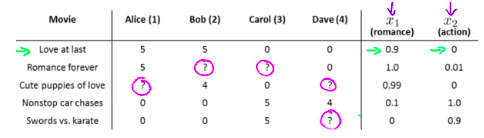
\includegraphics[width=\textwidth]{thesis/images/content_based_1.png}
\caption{Content-based Utility Matrix}
\end{figure}

Như ví dụ ở trên, ta đơn giản hóa bằng cách xây dựng vector đặc trưng cho mỗi bộ phim. Chiều thứ nhất của vector là độ lãng mạn (romance), chiều thứ 2 là mức độ hành động (action). Gọi các vector đặc trưng cho mỗi bộ phim là $x_1$, $x_2$, $x_3$, $x_4$, $x_5$ ta sẽ có giá trị mỗi vector là $x_1$ = [0.9, 0], $x_2$ = [1.0, 0.01], $x_3$ = [0.99, 0], $x_4$ = [0.1, 1.0], $x_5$ = [0, 0.9].

Tương tự, tính cách của mỗi người dùng cũng có thể được mô hình hóa dưới dạng tập các tham số $\theta$. Dữ liệu huấn luyện để xây dựng các mô hình $\theta$ là cặp item profile - rating tương ứng với các người dùng mà user đó đã đánh giá. Việc điền giá trị còn thiếu trong ma trận utility là dự đoán mức độ quan tâm khi áp dụng mô hình $\theta$ lên chúng. Đầu ra có thể viết dưới dạng f($\theta$,x). 

\subsection{Xây dựng hàm mất mát}
Giả sử số người dùng là N, số phim là M. Ma trận profile là X = [$x_1$, $x_2$,..., $x_m$] $ \in R_{d \times M}$ (d là số feature) và ma trận utility $Y \in R_{M \times N}$ Thành phần ở hàng thứ m, cột thứ n của Y là mức độ quan tâm của người dùng thứ n lên sản phẩm m mà hệ thống thu thập được. Giả sử tìm được 1 mô hình cho mỗi người dùng minh họa bởi vector $W_n \in R^d$ sao cho độ quan tâm có thể được tính theo công thức:
\begin{equation}
    y_{mn} = w^T_n x_m + b_n
\end{equation}

Xét user thứ n, coi training set là tập hợp các thành phần đã được điền của $y_n$, có thể xây dựng hàm mất mát tương tự như ridge regression:
\begin{equation}
    L_n(w_n,b_n)=\frac{1}{2s_n} \underset{m:r_{m n}}{\sum} (w^n x_m + b_n - y_{m n})^2 + 
    \frac{\lambda}{2s_n} \|w_n\|^2_2 
\end{equation}
trong đó, thành phần thứ hai là regularization và $\lambda$ là tham số dương, $s_n$ là số lượng các item mà user thứ n đã đánh giá.

Vì ở biểu thức trên $s_n$ là hằng số nên ta tập trung vào tối ưu phương trình đơn giản hơn dưới đây.
\begin{equation}
    \min \frac{1}{2} \underset{m:r_{m n}}{\sum} (w^n x_m + b_n - y_{m n})^2 + 
    \frac{\lambda}{2} \|w_n\|^2_2 
\end{equation}

Content-based recommendation system có điểm mạnh là không cần có data về những người dùng khác vì việc gợi ý chỉ tập trung vào từng người dùng. Điều này giúp cho việc scale lên một lượng user lớn trở nên dễ dàng hơn. Hơn nữa, model này có thể nắm bắt được sở thích của người dùng (VD thể loại phim hay xem, ca sĩ ưa thích, ...) và từ đó có thể gợi ích niche item mà ít người dùng thích.

Tuy nhiên, content-based recommendation system vẫn còn một số điểm yếu như sau. Vì phương pháp cần phải có feature của từng sản phẩm nên vẫn phụ thuộc vào độ chính xác của thông tin các feature này. Ngoài ra, model này chỉ có thể recommend dựa trên sở thích đã biết của người dùng. Nói cách khác, model này không thể gợi ý những sản phẩm nằm ngoài sở thích đã biết của người dùng.
